\newpage

\section*{ Rhodium }

Power Level: 100 kW(th) \\
Time at Power: 60 s \\
Wait Time: 3600 s \\
Total Activity at Removal: 4.02e+04 $\mu Ci$

\begin{table*}[h]
\centering
\begin{tabular}{ |c|c|c|c|c|c|c| }
 \hline
 Position & Mass $mg$ & Start Counting $s$ & Counting Time $s$ & Counting Activity $\mu Ci$ \\
 \hline 
 1 & 0.7 & 3660 & 600 & 1.95e+00\\ 
\hline
 2 & 0.55 & 4260 & 600 & 8.41e-01\\ 
\hline
 3 & 0.5 & 4860 & 600 & 5.79e-01\\ 
\hline
 4 & 0.55 & 5460 & 600 & 5.41e-01\\ 
\hline
\end{tabular}
\end{table*}

\begin{figure}[!ht]
   \centering
   \subfloat[][Position \#1]{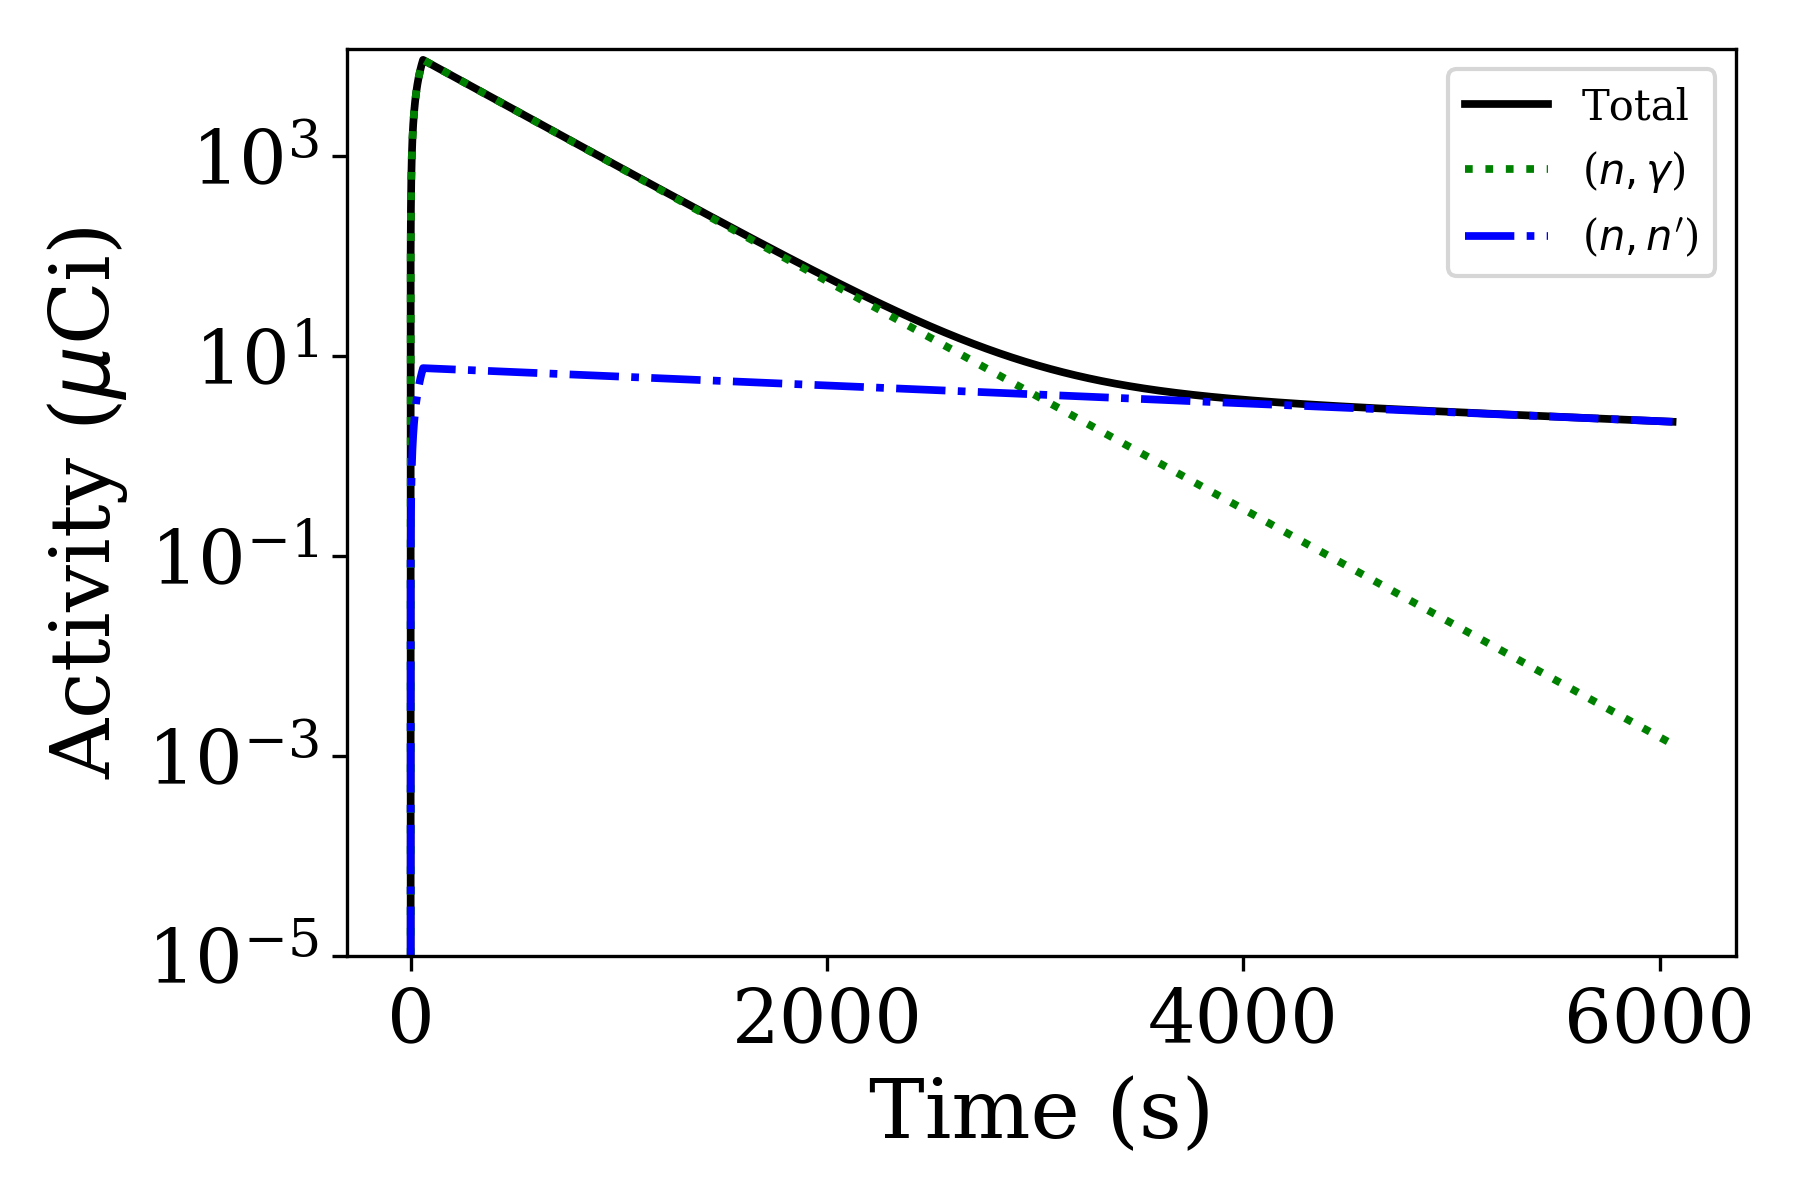
\includegraphics[width=.4\textwidth]{source/plot/rh1_activity}}\quad
   \subfloat[][ ($n,\gamma$) Reaction Rate]{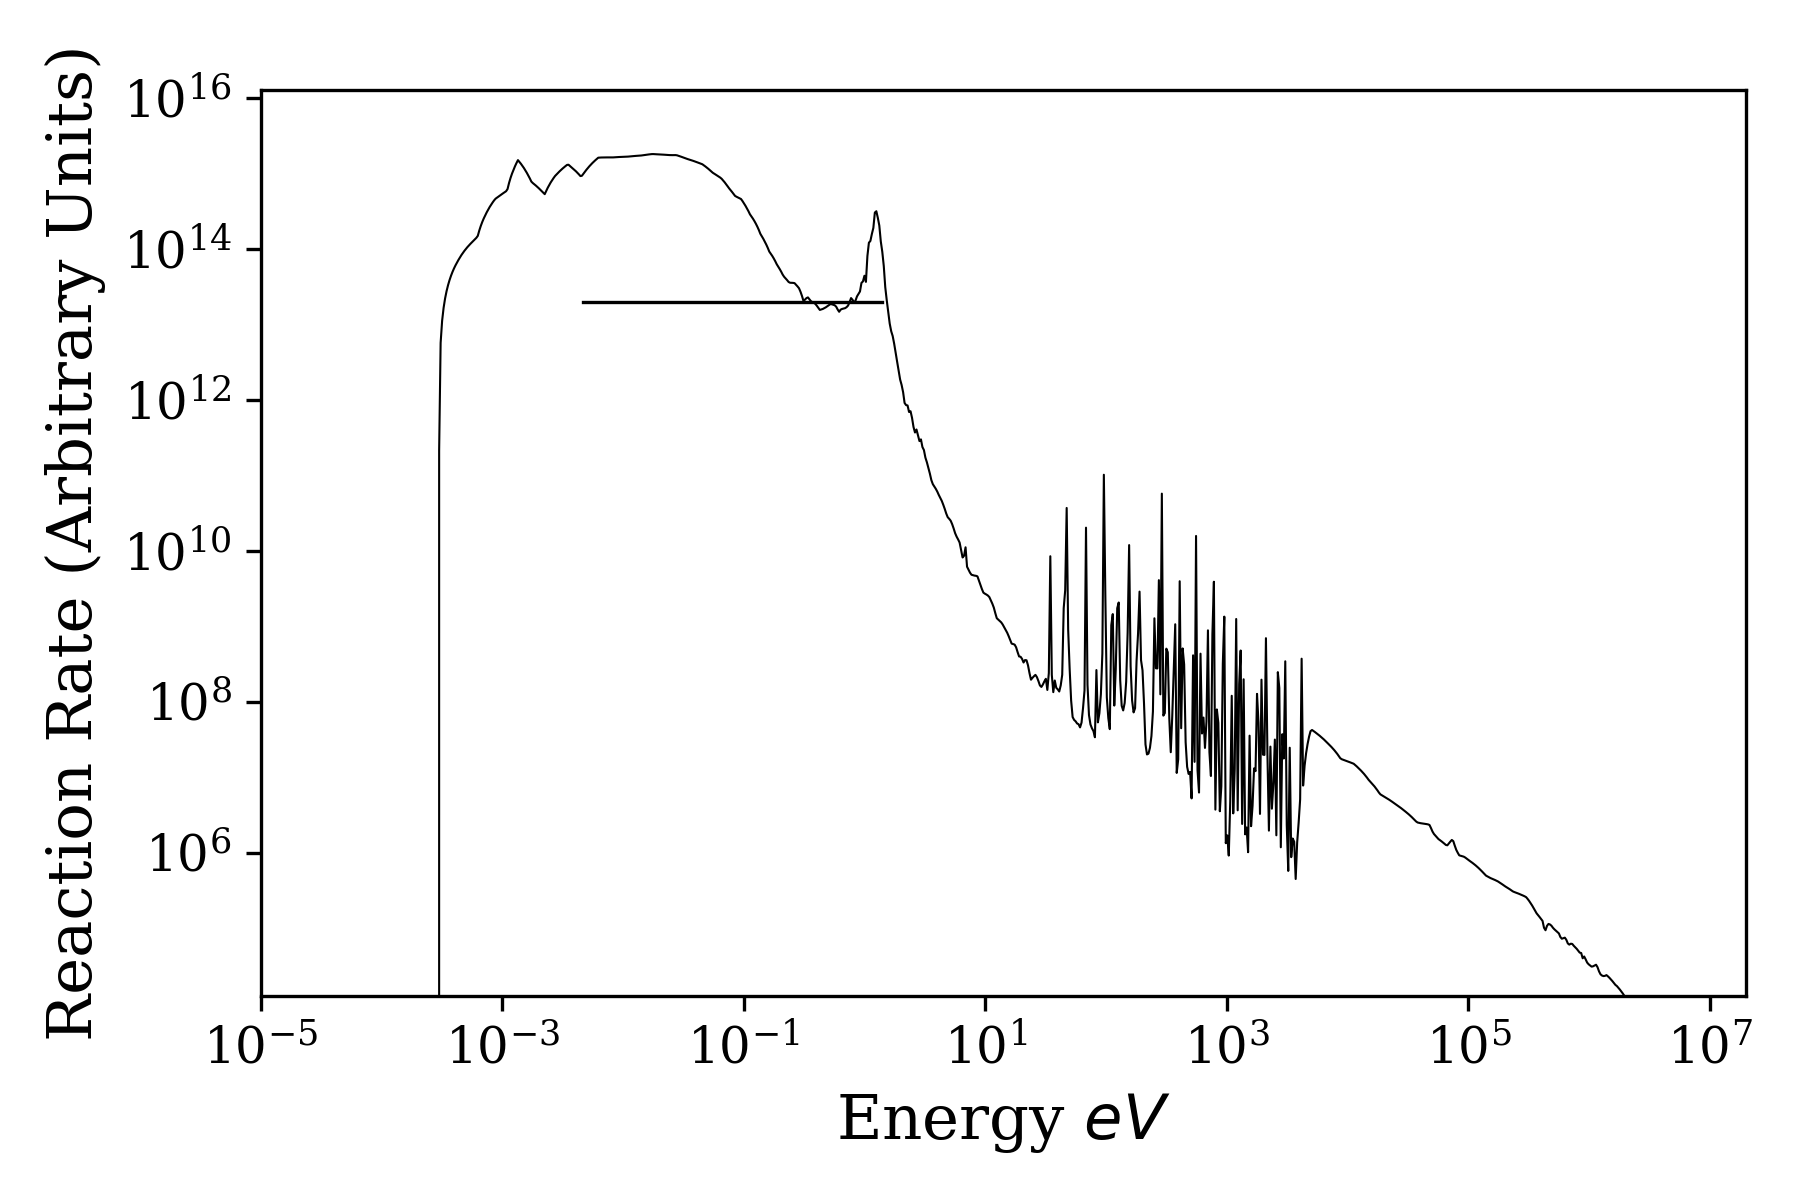
\includegraphics[width=.4\textwidth]{source/plot/rh_n,gamma}}\\ 
   \subfloat[][ ($n,n'$) Reaction Rate]{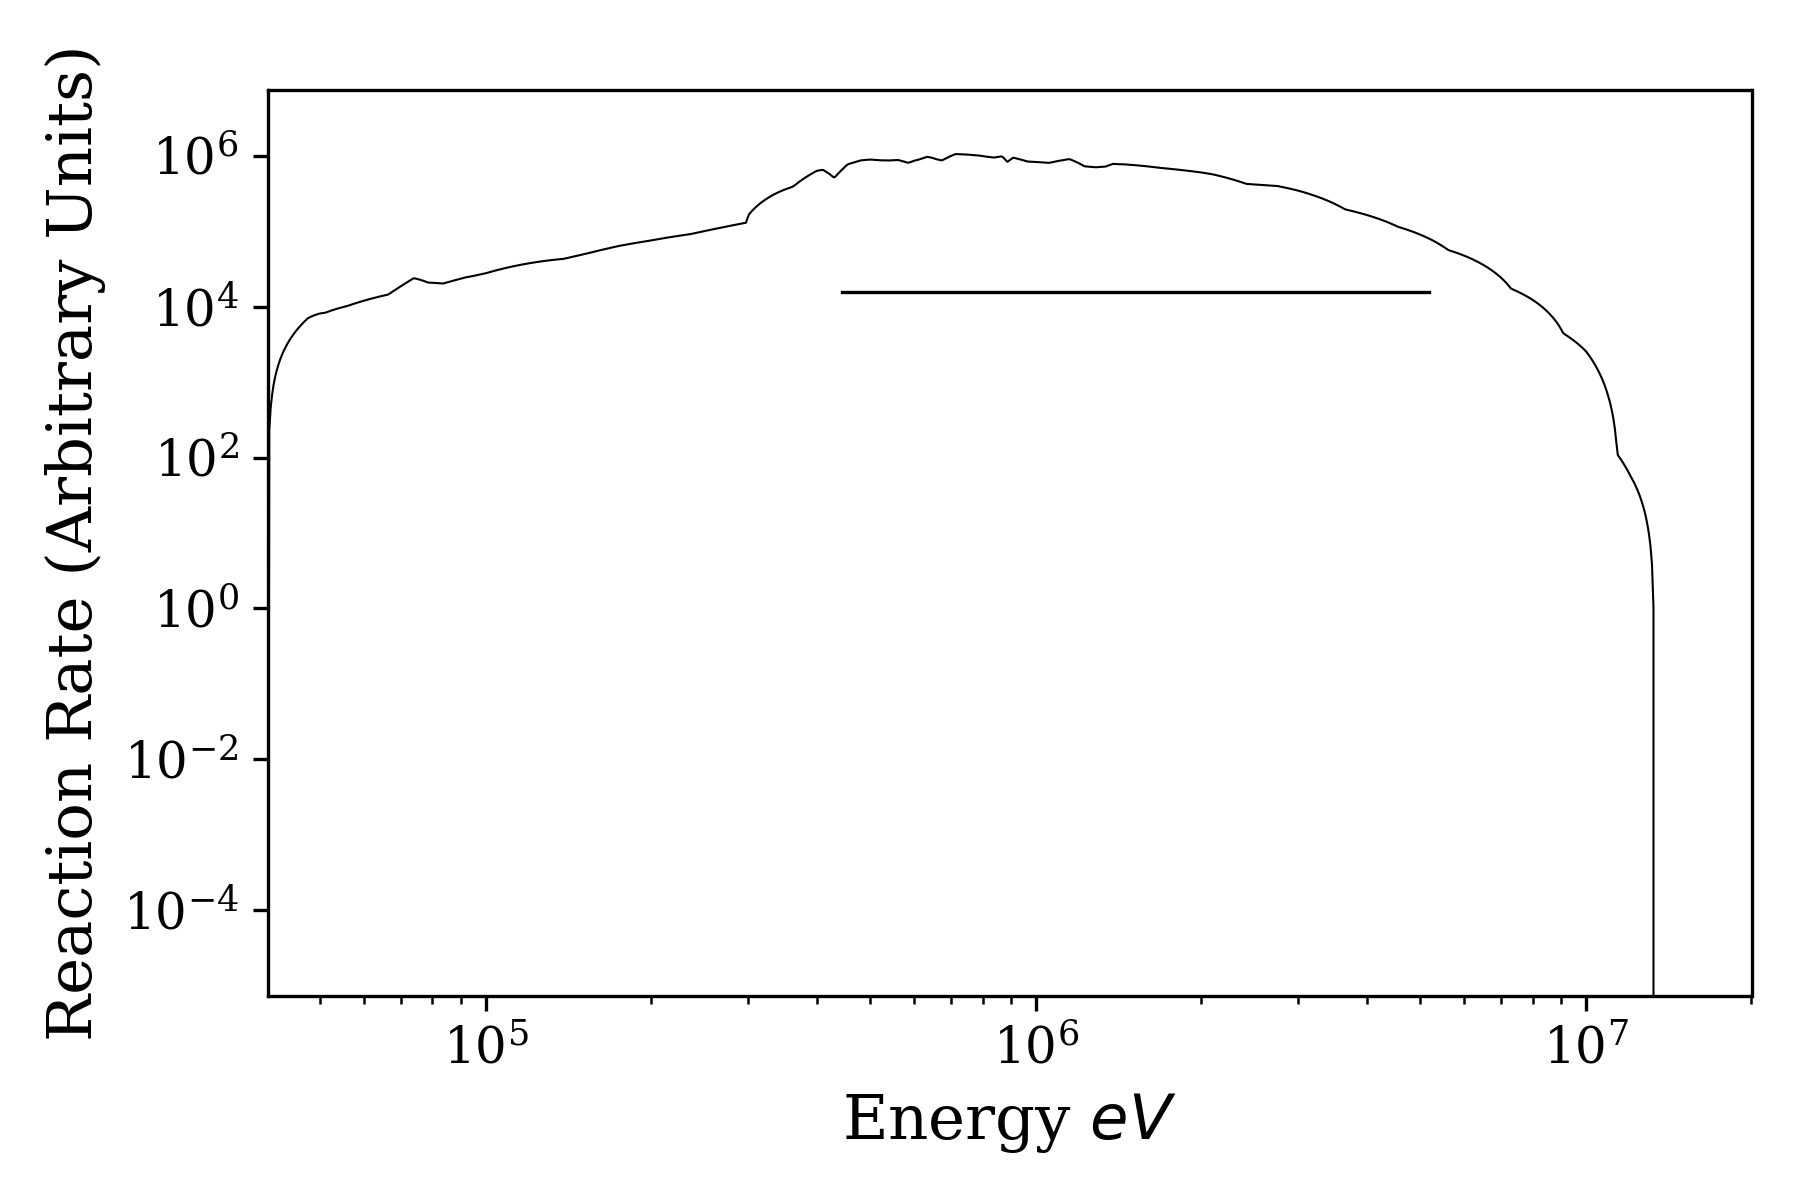
\includegraphics[width=.4\textwidth]{source/plot/rh_n,inelastic}}\quad 

\end{figure}

\begin{table*}[h]
\centering
\begin{tabular}{ |c|c|c|c|c|c|c| }
 \hline
 Reaction & T$_{1/2}$ & ROI (eV) & Important Gammas (keV) \\
 \hline 
 ($n,\gamma$) &  4.4 m & 4.67e-03, 1.39e+00 & 51(0.47), 78(0.025), 560(0.026), 770(0.0018) \\ 
\hline
 ($n,n'$) & 56.1 m & 4.45e+05, 5.19e+06 & 40(0.004) \\ 
\hline
\end{tabular}
\end{table*}
